\documentclass[final,5p,times,twocolumn,numbers]{elsarticle}
\usepackage{amsmath,amssymb,booktabs,tabularx,graphicx,microtype,xurl}
\usepackage{tikz}
\usetikzlibrary{positioning,arrows.meta}
\usepackage[hidelinks]{hyperref}
\usepackage{placeins,flushend}
\hypersetup{pdfauthor={Zhichao Zhang, Daoqi Sun, Xiaolu Peng},pdftitle={RePressDB: Risk-Aware Layout Adaptation with Efficient Durable Replacement}}
\journal{Future Generation Computer Systems}
\biboptions{numbers,sort&compress}
\graphicspath{{figures/}{./}}
\setlength{\emergencystretch}{2em}
\setlength{\textfloatsep}{11pt plus 2pt minus 2pt}
\setlength{\floatsep}{9pt plus 2pt minus 2pt}
\raggedbottom
\begin{document}
\begin{frontmatter}
\title{RePressDB: Risk-Aware Layout Adaptation with Efficient Durable Replacement}
\author[aff1]{Zhichao Zhang\corref{cor1}}
\ead{zhichao.zhang2024@outlook.com}
\author[aff1]{Daoqi Sun}
\ead{sundao0217@gmail.com}
\author[aff2]{Xiaolu Peng}
\ead{lilypxl1656179423@outlook.com}
\cortext[cor1]{Corresponding author: Zhichao Zhang (zhichao.zhang2024@outlook.com).}
\address[aff1]{School of Science, Minzu University of China, No. 27 Zhongguancun South Avenue, Beijing, 100081, China}
\address[aff2]{School of Navigation, Dalian Maritime University, No. 1 Linghai Road, Ganjingzi District, Dalian 116026, China}


\begin{abstract}
Changing query mixtures can alter the preferred compressed layout of immutable time-series chunks, but online adaptation must balance query-latency risk against the cost of durable replacement. We present RePressDB, a file-backed storage component that coordinates empirical tail admission with recoverable reconfiguration. The controller models latency by query operation and range length, filters candidates through calibrated tail distributions, and accumulates benefit evidence within consecutive feasible decision epochs. Admission prices installation and a possible return to the reference layout. Conditional-distribution count tables reduce decision overhead, while a three-transaction catalog path preserves atomic activation and ordered retirement. Six policies share a common executor over 23.04 million checked queries and 24 workload instances. Compared with a cumulative-credit controller, RePressDB reduces migrations from 155 to 66 and target rewriting from 5.595 to 2.375~MiB. Its event-p99 ratio is 0.872 (95\% interval 0.816--0.928), with a service-time ratio of 1.029 (0.995--1.065). Under persistent workload shifts, service time is 25.0\% lower than a fixed initial layout. The revised executor has a median paired migration-time ratio of 0.786 against the six-transaction path, and all 492 software-fault trials pass. The measurements characterize how query mixture, its persistence, and the full action path determine the value of adaptation.

\end{abstract}
\begin{keyword}
time-series storage \sep online physical design \sep adaptive compression \sep switching cost \sep runtime reconfiguration \sep crash recovery
\end{keyword}
\end{frontmatter}
\section{Introduction}
Time-series services execute point retrievals, scans, and aggregates over immutable measurements. These operations favor different compressed layouts: small blocks limit decompression for selective requests, while whole-chunk compression reduces block-processing work for broad scans. The preferred representation can therefore change with the request mixture even when the values remain fixed.

Replacing that representation affects both query execution and maintenance. A layout with a lower average query cost may expose a costly minority of operations. Installation also requires file synchronization, validation, catalog activation, and cleanup. If a later mixture makes the accepted layout unattractive, returning to a reference layout adds another directed replacement. These costs connect the duration of the workload evidence to the physical action it supports.

Existing research addresses distinct parts of this decision. Online physical design, including OReO, balances query processing and reorganization through switching-cost models and layout generation \citep{rong2024oreo}. Adaptive compression, including AdaCom, changes segment compression according to access statistics and memory/CPU trade-offs \citep{windheuser2024adacom}. Transaction and versioning mechanisms establish atomic visibility and recovery for persistent state \citep{mohan1992aries,gray1992transaction,sqlitewal}. For compressed immutable chunks, these concerns meet at an operation-dependent query path and an executed file replacement. The query distribution used for admission must be interpreted alongside the cost and recovery boundary of that action.

This leads to the research question: \emph{When should a storage component replace a compressed layout under an evolving query mixture, accounting for operation-dependent latency distributions, durable replacement cost, and a possible return to a reference layout?} A sustained favorable mixture can provide time to recover the action cost; evidence retained across separate feasible periods can instead support a late or repeatedly reversed change. Recent work on index-tuning regressions similarly motivates examining the query behavior behind an estimated average benefit \citep{wu2025qpr}.

We present RePressDB, a file-backed component that coordinates layout admission and recoverable physical replacement. The controller separates query operations and range lengths, filters layouts through empirical tail distributions, and accumulates advantage over consecutive feasible decision epochs. Admission prices both installation and return to the reference layout. The executor measures and performs the complete replacement, groups catalog changes around reservation, activation, and retirement, and commits retirement before deleting old files. Conditional-distribution count tables make the empirical filter practical on the request path.

The contributions are:
\begin{enumerate}
\item A risk- and switching-cost-aware admission mechanism linking operation/length distributions, consecutive feasible decision epochs, and directed installation-plus-return prices. The link determines which observed opportunities can justify a physical change as query mixtures evolve.
\item A low-overhead, recoverable execution design combining exact conditional-count decisions with a three-transaction replacement path. Its visibility and retirement boundaries support a recovery case split and measurement of complete action cost.
\item A common-executor study that separates control-policy trade-offs from executor improvements. Shared inputs, layouts, budgets, and timing boundaries support joint interpretation of service, event tails, controller work, and rewriting; decision and post-action analyses explain the conditions encountered by the mechanism.
\end{enumerate}

\section{Problem and cost boundary}
\label{sec:problem}
The managed unit is an immutable one-dimensional chunk of little-endian float32 values. Layouts are whole-chunk LZ4, whole-chunk Zstandard level~3, and LZ4 blocks of 64, 256, 1,024, or 4,096 values. The additional 4,096-value layout exposes an intermediate selective-decompression cost. Every policy receives the same six-layout action space.

The query interface supports points, scans, sums, averages, minima, maxima, and threshold counts. Range lengths span 0.1\%, 1\%, 10\%, 50\%, and 100\% in the workload generator; threshold requests use its three supported lengths. A scan consumes the selected values and returns their float64 sum. The evaluated component supports immutable-chunk replacement and sequential request execution.

For a request sequence, modeled cost is
\begin{equation}
C=\sum_{t=1}^{T}\mu_{c_t}(r_{c_t,t},x_t)+\sum_{e\in\mathcal M}m_{c_e}(r_e^-,r_e^+),
\label{eq:cost}
\end{equation}
where $\mu$ is calibrated query-path mean cost and $m$ is complete directed replacement cost. Measured service additionally contains controller work and view reconstruction. Calibration is a commissioning expenditure reported separately. Event quantiles assess the distribution of query, controller, and synchronous maintenance cost together.

\section{Risk-aware layout admission}
\label{sec:admission}
\subsection{Operation and length cost distributions}
A point lookup, a broad scan, and a range aggregate exercise different compressed-data paths. Aggregates also differ by operation: a block sum can use its summary, whereas a threshold count may decompress ambiguous blocks. RePressDB describes a request by $x=(o,b)$, its operation and normalized range-length bin. Operations are point, scan, sum, average, minimum, maximum, and threshold count. Length-bin upper boundaries are $0.002$, $0.02$, $0.2$, $0.75$, and $1$. Points occupy a separate stratum; the evaluated interface populates 29 strata.

Calibration executes 64 measured queries per chunk/layout/stratum after four warmups. Positions and threshold values cycle through shuffled complete stratum pools. All latency samples $z_{c,r,x,j}$ and their means $\mu_c(r,x)$ are retained. Every policy receives this cost surface. Admission additionally uses the empirical distributions. For recent weights $w(x)$,
\begin{align}
\widehat L_{c,w}(r)&=\sum_xw(x)\mu_c(r,x),\\
\widehat F_{c,w,r}(u)&=\sum_x\frac{w(x)}{64}\sum_{j=1}^{64}\mathbf1[z_{c,r,x,j}\leq u].
\end{align}

\subsection{Tail admission and risk repair}
Let $a_0$ be a chunk's common initial layout. Its empirical 99th percentile under each current mixture defines
\begin{equation}
\tau_{c,w}=1.10\inf\{u:\widehat F_{c,w,a_0}(u)\geq0.99\}.
\end{equation}
The 10\% tolerance is fixed before the comparison. Feasible candidates satisfy
\begin{equation}
\mathcal F_c=\{r:1-\widehat F_{c,w,r}(\tau_{c,w})\leq0.01,\ w\in\{s,l\}\}.
\label{eq:feasible}
\end{equation}
Equation~\eqref{eq:feasible} is an empirical filter on calibrated query-path risk under the observed mixture. Measured event latency additionally charges controller work and synchronous replacement. The initial layout remains available. Short and long windows contain 256 and 768 local queries. Their block histograms supply feature weights. The target must minimize estimated mean cost within $\mathcal F_c$ in both windows, improve the active layout by at least 8\% in each, and persist for three rounds. An expensive minority of requests therefore affects admission before an average-cost improvement is accepted.

When the active layout fails Eq.~\eqref{eq:feasible}, the reference layout becomes a risk-repair target with a two-round target-confirmation threshold. Risk repair uses the same executor and byte budget. Its full cost remains in service timing. The gate evaluates calibrated query-path distributions; measured event tails additionally contain control work and maintenance.

\subsection{Blockwise action evidence}
A feasible epoch is a sequence of consecutive decision boundaries at which a candidate passes Eq.~\eqref{eq:feasible}. Each 256-query block supplies one empirical mixture observation. Each query updates one feature count, and histogram $h_k(x)$ updates advantage at the boundary. Let $D_k(r)=\sum_xh_k(x)[\mu_c(a,x)-\mu_c(r,x)]$. Then
\begin{equation}
A_k(r)=\begin{cases}
\max\{0,A_{k-1}(r)+D_k(r)\},&r\in\mathcal F_c,\\
0,&r\notin\mathcal F_c.
\end{cases}
\label{eq:credit}
\end{equation}
A feasible target passing the persistence tests is admitted when
\begin{equation}
A_k(r^*)\geq1.25[m_c(a,r^*)+m_c(r^*,a_0)].
\label{eq:admission}
\end{equation}
A change resets counters and starts a 768-query cooldown. Initial incomplete windows supply zero credit. An infeasible interval discards a target's old evidence, so a later favorable regime must rebuild it. The price includes a directed return to the reference layout, accounting for the repair that a later mixture may require. This couples action evidence to the controller's own return behavior. The rule uses historical advantage as a conservative admission heuristic. Subsequent query mixtures determine how much of that opportunity becomes post-action saving. Return pricing raises the evidence threshold; the byte budget is checked when each actual action is proposed.

\textit{Block evidence property.} For a fixed active layout and common reset points, Eq.~\eqref{eq:credit} is bounded above by the corresponding counter reflected after every request. Successive updates $v\mapsto\max(0,v+d_i)$ yield at least $\max(0,v+\sum_i d_i)$ for a block's increments. Induction over blocks gives the result. Resets at infeasible epochs preserve the inequality. Thus batching and epoch resets supply conservative boundary evidence and reduce per-request arithmetic.

Request accounting costs $O(1)$. Three histograms require $O(K)$ state. Repeatedly scanning $RKS$ latency samples at a decision boundary can itself affect event tails. We therefore prepare conditional-distribution counts once from the calibration samples. Let $U$ be the number of distinct initial-layout sample latencies. For every such value $u$, we store the initial layout's per-feature counts at $u$ and each candidate's exceedance counts at $1.10u$. Each count fits in one byte because $S=64$.

The initial-layout empirical quantile lies on this finite support. Binary search over its weighted conditional counts locates the reference value, and a matrix-vector product supplies each candidate's exceedance probability. This evaluates the same empirical criterion with $O(K\log U+RK)$ decision work and $O(RKU+KU)$ bytes of count tables. Sample sorting and table construction are commissioning work; their measured initialization cost is reported separately. Distribution lookup and decision logging remain inside the controller timer.

An implementation-equivalence check replays all 2.88 million requests from the preceding frozen evaluation. All 11,181 decision boundaries, counters, proposals, and recorded actions agree. Alternating-order component timings compare the scanning and count-table implementations, preserving their setup measurements as a separate expenditure.

\subsection{Shared payload budget}
Every policy enforces, per 1,000 global queries,
\begin{equation}
\sum_{e\in\mathcal M_k}b_{c_e}(r_e^-,r_e^+)\leq B_k.
\label{eq:budget}
\end{equation}
Here $B_k$ equals the largest calibrated candidate payload plus metadata in the instance. Deferred proposals face subsequent evidence and risk checks. This measure covers target files; journals and device write amplification require separate accounting. In the final Risk-RePress runs, the limit deferred one proposal. Section~\ref{sec:mechanism} reports this execution constraint alongside the other decision outcomes.

\section{Three-transaction durable replacement}
\label{sec:execution}
A catalog row names one active immutable version, its codec, paths, sizes, checksum, and an optional retained previous version. SQLite uses WAL with \texttt{synchronous=FULL}. A process-local lock serializes replacement and view changes.

The original path committed intent, encoding, validation, publication, activation, and cleanup in six transactions. The revised path uses three durable recovery decisions:
\begin{enumerate}
\item \textit{Reserve.} $T_1$ records source and target versions and every temporary and final candidate pathname. Decode, encode, synchronization, validation, and file publication proceed locally while the source remains active.
\item \textit{Activate.} $T_2$ atomically installs the validated target, retains its predecessor, and records committed-pending-cleanup state. The active view is invalidated and the catalog-visible version is validated.
\item \textit{Retire.} $T_3$ clears the previous-version pointer and completes the migration log. Physical deletion follows; startup sweeping collects interrupted deletion's unreferenced files.
\end{enumerate}

Retirement ordering matters for block layouts. Reconstructing a retained version requires its metadata. Deleting that metadata while the catalog still refers to it can break restart cleanup. Committing retirement first makes partially deleted old files unreferenced garbage while preserving the validated active version.

Figure~\ref{fig:lifecycle} connects three parts of the component. Panel~A shows query-path admission: normal candidates pass the two-window target, gain, confirmation, evidence-price, and cooldown conditions, while risk repair returns to the reference layout after two confirmations. Both paths check the shared payload budget; deferred proposals retain the active layout and are reconsidered at later decisions. Panel~B shows the successful transactional replacement, and panel~C identifies restart actions before activation, while a predecessor is retained, and after retirement.

\begin{figure*}[t]
\centering
\includegraphics[width=\textwidth]{fig1_image.png}
\caption{RePressDB admission, replacement, and recovery.}
\label{fig:lifecycle}
\end{figure*}

Before $T_2$, recovery retains the source and removes $T_1$'s candidate paths. Between $T_2$ and $T_3$, a valid target completes retirement; an invalid target can be replaced by the retained checksum-valid source. After $T_3$, the target is authoritative and remaining old files are garbage. Repeated cleanup reaches the same active pointer and file set. This case split covers partial payload/metadata publication because activation follows validation of both files.


\begin{table}[t]
\centering\small
\caption{Recovery states at transaction boundaries.}
\label{tab:invariants}
\begin{tabularx}{\columnwidth}{@{}lccX@{}}\toprule
Interval & Active & Retained & Restart action \\
\midrule
$[T_1,T_2)$ & $a$ & -- & Keep $a$; discard candidate paths. \\
$[T_2,T_3)$ & $r$ & $a$ & Validate $r$; finish retirement or restore valid $a$. \\
After $T_3$ & $r$ & -- & Keep validated $r$; collect unreferenced files. \\
\bottomrule\end{tabularx}
\end{table}

Table~\ref{tab:invariants} summarizes the recovery case split. Payload synchronization and pre- and post-activation validation remain in the path. Fault tests exercise ten software-visible stages, abrupt exits, and corruption while a previous version is retained. Windows/NTFS is the measured persistence environment; hardware and device ordering determine additional deployment properties.

The shared active view retains the catalog row, parsed metadata, representation object, and open handles. Queries execute the file-backed codec path. Migration, recovery, rollback, creation, and close invalidate views; reconstruction after activation is charged to the next query. All policies use this view and executor. Directed calibration includes decode, encode, synchronization, validation, activation, retirement, and deletion. Independent truth checks run outside query timers. Per-event arrays preserve query, control, and maintenance time.

\section{Evaluation}
\label{sec:evaluation}
The evaluation asks: (RQ1) how much work is saved by consolidating durable preparation stages; (RQ2) how risk-aware admission changes service time, tails, and rewriting under common execution; and (RQ3) how the revised path recovers across its publication and retirement boundaries.

\subsection{Evidence roles and data}
The new policy comparison uses 24 Building Data Genome~2 building-meter series \citep{miller2020bdg2}, partitioned into three groups of eight. The earlier eight-building timing subset is excluded. These 24 buildings appeared in earlier replay and in the development campaign used to identify the method's weaknesses. The new campaign uses fresh request seeds, frozen method parameters, and new calibration; its role is a subsequent evaluation on this measured corpus.

Each building supplies paired 8,192- and 16,384-value chunks. The 48 distinct chunks contain 2.25~MiB of raw values. Reconstructed bytes match archived raw SHA-256 values. The experiment characterizes a warm working set and file-backed codec execution. The data and query roles remain explicit: measurements are real building data, while requests come from semi-synthetic continuous mixtures.

The final method and parameters were frozen before the reported execution. The physical corpus had already been used during development; recorded request seeds define subsequent evaluations on that corpus. Six policies share the final inputs and executor. Development records, source changes, and the complete implementation-equivalence audit are retained in the reproducibility archive.

\subsection{Requests, layout space, and common inputs}
Gradual-periodic, mean-reverting, and noisy-burst families change the relative weights of point, scan, and aggregate requests continuously. A fourth, persistent-shift family characterizes a longer opportunity to recover replacement cost. Its first 20,000 requests use the fixed initial scan-heavy weights. The remaining 140,000 use weights 0.94, 0.025, 0.005, 0.0005, 0.01, 0.005, 0.01, and 0.0045 for point, short/medium/long scan, short/medium/long aggregate, and threshold requests, respectively. This family was specified before the final execution, and its six instances are reported separately from the 18 continuous-mixture instances. Each group/size/family instance contains 160,000 requests. A seeded skewed distribution selects chunks, and seeded draws select query classes and concrete arguments. The seed list is recorded before calibration and policy execution.

The design contains 24 instances and six policies, producing 144 executions and 23.04 million events. All policies receive the same concrete requests, six layouts, initial layout, empirical query-cost means, complete migration table, read path, and payload-write budget. The initial layout minimizes calibrated scan-heavy cost, using the same fixed deployment-time weights. Feature weights expand these class weights according to the query pool's operation/length proportions.

\subsection{Compared policies}
\textit{Static} retains the common initial layout.

\textit{Shape-EWMA-BE} tracks the common operation/length features using EWMA $\alpha=0.01$, a 5\% deadband, a 300-query projection horizon, 100-query decision intervals, and 200 initial observations. The settings come from the earlier PEMS04 development protocol.

\textit{Horizon-RePress} retains 300/100-query windows, 8\% gain, three confirmations, a 300-query cooldown, a 1,200-query projection, and a 1.25 cost margin. In this campaign it uses the same refined query means and full three-transaction migration prices as every adaptive policy.

\textit{Work-function-inspired} (labelled Work-function in tables and figures) maintains one value per layout over the common six-layout space at 100-query boundaries:
\begin{equation}
W'(r)=v(r)+\min_s\{W(s)+m(s,r)\}.
\end{equation}
Here $v(r)$ sums the block's calibrated feature costs. A common minimum is subtracted for stability. The policy proposes the minimizer of $W'(r)+m(a,r)$, starting with directed costs from the initial layout \citep{azar2007workfunction}. Directed measured prices, six fixed layouts, block decisions, and the common budget define this switching-cost baseline. OReO additionally provides a layout generator and a theoretical framework for its own action model.

\textit{Credit-RePress} retains the previous per-request reflected counter, 300/100-query windows, three confirmations, 8\% gain, 300-query cooldown, and 1.25 cost threshold. Its profile is expanded to the common operation/length features. This comparison tests the revised controller against accumulated admission under the same expanded inputs and executor.

\textit{Risk-RePress} implements Section~\ref{sec:admission}: 256-query blocks, three-block long windows, a 10\% empirical tail tolerance, epoch-bound advantage, forward-plus-return action prices, and budgeted risk repair. These settings were frozen before this comparison. The comparison measures complete operating policies; paired executor measurements isolate the change to durable execution separately.

\subsection{Calibration, timing, and correctness}
Calibration measures 64 queries after four warmups for each chunk/layout/feature stratum. Layout order rotates between chunks, and complete stratum pools are shuffled with recorded seeds. All 8,352 records retain raw samples, means, medians, and p95 values. Three complete replacements measure each nontrivial directed layout pair, giving 4,320 observations. Setup replacements are included in calibration wall time and excluded from policy action counts.

Every timed execution uses a fresh store and prewarms one query per chunk. Only one performance worker runs at a time, pinned to logical processor~0. Policy order rotates cyclically across the 24 instances, so every policy occupies each position four times. Query, controller, and migration arrays are stored separately. Event service is
\begin{equation}
L_t=T_{\mathrm{query},t}+T_{\mathrm{control},t}+T_{\mathrm{migration},t}.
\end{equation}
Controller timing includes feature extraction, distribution calculations, decision logging, and successful-switch state updates. Queries after migration include active-view reconstruction. The triggering event pays for synchronous maintenance. Network transport and arrival-process queuing require additional service models.

Every result is checked independently against raw float32 values outside service timers. Integer results use exact equality; floating results use relative tolerance $10^{-7}$ and absolute tolerance $10^{-5}$. Final decoded arrays must match exactly, and catalog integrity must pass in each cell.

The host is an Intel Core i7-14700HX Windows/NTFS system with approximately 16~GB memory and NVMe storage. Execution uses Python~3.10.20, NumPy~2.2.6, Pandas~2.3.3, LZ4~4.4.5, and Zstandard~0.25.0. Sources, calibration, parameters, environment, event arrays, and decisions are preserved with hashes. Locally executed code supplies all measurements.

\subsection{Analysis}
Controller initialization, including conditional-count table construction, is measured separately from steady-state service. Passive host observations are preserved alongside the execution log.

The new analyses reuse recorded decisions, query features, event components, and the frozen cost surface. Gate outcomes are reconstructed in execution order and checked against logged proposals, committed migrations, and budget deferrals. For each migration, calibrated query-cost differences over the subsequent observed episode are compared with measured action cost. Stable-window analysis keeps model feasibility, observed query p99, and observed event p99 as separate quantities. The analysis archive binds every input file by SHA-256.

The paired unit is a group/size/family instance. We report equal-weight geometric-mean ratios, win counts, and percentile-bootstrap 95\% intervals from 20,000 paired instance resamples. These summaries describe generated request variation conditional on the corpus, fixed calibration, and host. Every scheduled final cell is retained. Continuous and persistent-shift strata are reported separately, with their own paired summaries. Intervals spanning one express the range of effects supported by this experiment. Migrations and target bytes are also reported as campaign totals.

\section{Results}
\label{sec:results}
\subsection{RQ1: Replacement and decision work}
All six policy executions use the revised three-transaction executor. The six-versus-three transaction comparison is a separate paired diagnostic. It selects the first two manifest-ordered chunks in the first building group at each size. Four chunks cover 80 nontrivial directed pairs over the five original layouts. Each pair has three repetitions; execution order alternates between the original and revised executor using independent stores. Target payload and metadata bytes match in every observation. SQL trace callbacks record six COMMIT statements for the original path and three for the revised path.

Across directed-pair medians, the original and revised replacement times are 49.83 and 39.61~ms. The median paired ratio is 0.786, with 10th and 90th percentiles 0.724 and 0.828. Figure~\ref{fig:executor}(a) plots the 80 directed-pair medians from 240 observations; its dashed line marks equal time and 8K/16K count float32 values. Panel~(b) plots the cumulative distribution of three-transaction/six-transaction time ratios. Validation and file synchronization remain inside both measurements.


\begin{figure*}[!t]
\centering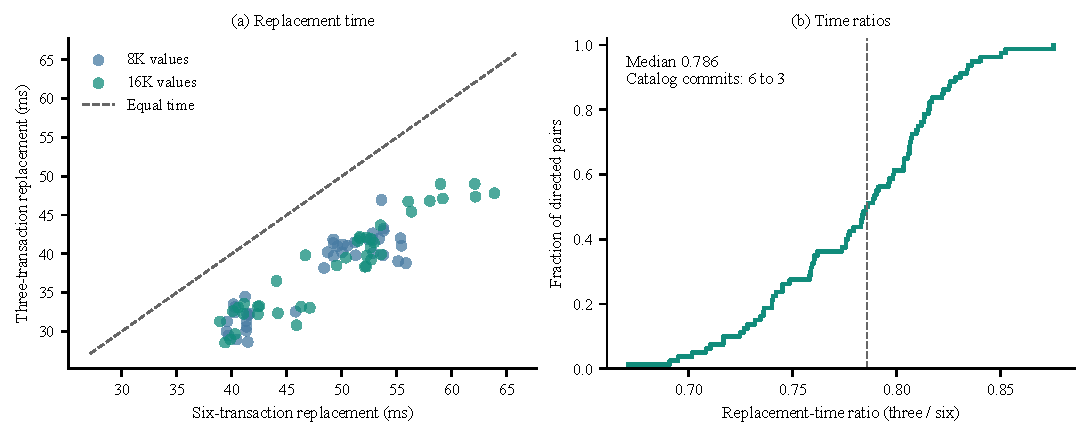
\includegraphics[width=.94\textwidth]{executor_cost.pdf}
\caption{Paired replacement costs.}
\label{fig:executor}
\end{figure*}
The equivalent count-table controller reduces median decision-boundary work from 90.1 to 47.1~$\mu$s in the alternating-order component diagnostic. Its median paired ratio is 0.523. All 2.88 million checked requests preserve the scanning implementation's decisions, counters, and recorded actions. In the final executions, controller initialization has a median of 8.69~ms and a maximum of 12.88~ms per eight-chunk instance. The additional conditional-count arrays have a median footprint of 0.363~MiB per instance.

The shared refined calibration completes 8,352 query-cost strata and 4,320 directed replacement observations. Its wall time is 400.9~s, including setup replacements. This commissioning expenditure is separate from the following steady-state policy measurements.


\subsection{RQ2: Selective migration and its service trade-off}
All 144 scheduled executions complete with 23,040,000 independently checked events, valid final arrays, and catalog integrity. All control policies share the revised executor; the separate diagnostic above measures the executor change. Tables~\ref{tab:newresults} and~\ref{tab:strata} retain every policy and both workload strata. Ratios are equal-weight geometric means, and brackets give paired-bootstrap 95\% intervals. Table~\ref{tab:newresults} uses Static as the denominator; rewriting includes target payloads and representation metadata.
\begin{table*}[!t]
\centering\small
\caption{Overall policy comparison.}
\label{tab:newresults}
\begin{tabular}{@{}lrrrrrr@{}}
\toprule
Policy & Service ratio & 95\% interval & Event p99 ratio & Migrations & Rewrite (MiB) & Control (\%) \\
\midrule
Static & 1.000 & -- & 1.000 & 0 & 0.000 & 0.00 \\
Shape-EWMA-BE & 1.054 & [1.025, 1.085] & 1.038 & 0 & 0.000 & 3.81 \\
Horizon-RePress & 0.998 & [0.934, 1.044] & 1.126 & 35 & 1.426 & 3.15 \\
Work-function & 1.007 & [0.971, 1.042] & 1.054 & 13 & 0.510 & 2.34 \\
Credit-RePress & 0.920 & [0.853, 0.986] & 1.264 & 155 & 5.595 & 5.16 \\
Risk-RePress & 0.947 & [0.884, 1.005] & 1.102 & 66 & 2.375 & 2.04 \\
\bottomrule
\end{tabular}
\end{table*}

\begin{table*}[!t]
\centering\small
\caption{Results by workload stratum.}
\label{tab:strata}
\begin{tabular}{@{}lrrrr@{}}\toprule
Stratum & Service / Static & Event p99 / Static & Service / Credit & Event p99 / Credit \\
\midrule
Continuous (18) & 1.023 [0.995, 1.052] & 1.140 [1.101, 1.184] & 1.026 [0.989, 1.066] & 0.825 [0.769, 0.880] \\
Persistent (6) & 0.750 [0.668, 0.830] & 0.997 [0.926, 1.053] & 1.039 [0.966, 1.110] & 1.033 [1.000, 1.068] \\
\bottomrule\end{tabular}
\end{table*}


Against Credit-RePress under identical calibrated inputs, Risk-RePress reduces migrations from 155 to 66 (57.4\%) and target rewriting from 5.595 to 2.375~MiB (57.5\%, computed from unrounded bytes). Its event-p99 ratio is 0.872 (95\% interval 0.816--0.928), with lower p99 in 20 of 24 instances. Its service-time ratio is 1.029 (0.995--1.065), placing the observed tail and rewrite reductions alongside the range of average-cost effects. Controller execution accounts for 2.04\% of Risk-RePress service and 5.16\% of Credit-RePress service. Figure~\ref{fig:comparison} plots service-time ratios in (a) and event-p99 ratios in (b), with paired-bootstrap 95\% intervals across 24 instances. Each row uses its named baseline as the denominator; ratios below one favor Risk-RePress. Event timing includes query, controller, and synchronous maintenance work, while admission evaluates calibrated query-path distributions. Work-function denotes the work-function-inspired baseline.

\FloatBarrier
\begin{figure*}[!t]
\centering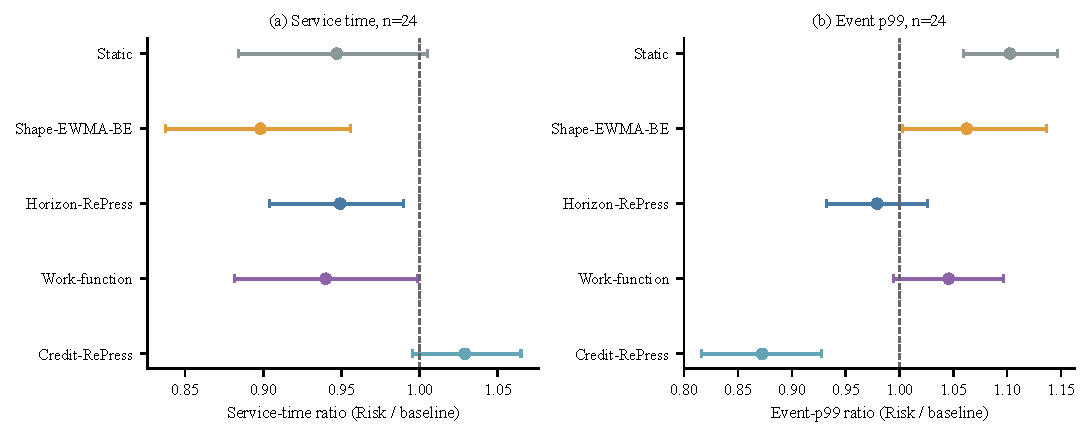
\includegraphics[width=.94\textwidth]{policy_comparison.pdf}
\caption{Service and event-tail comparisons.}
\label{fig:comparison}
\end{figure*}

The fixed-layout comparison addresses when adaptation pays. Under persistent shifts, Risk-RePress has a service ratio to Static of 0.750 (0.668--0.830), with a p99 ratio of 0.997 (0.926--1.053). Under continuous mixtures, the corresponding ratios are 1.023 (0.995--1.052) and 1.140 (1.101--1.184). A long point-heavy interval provides a different opportunity from repeated mixture changes. Panels (a,c) of Figure~\ref{fig:trajectories} show cumulative service relative to Static; panels (b,d) use Credit-RePress. Dotted lines in (c,d) identify the 20,000-query workload shift. Lines are geometric means; shading spans the 25th--75th percentiles across instances. Panels (a,b) use 18 continuous-mixture instances and (c,d) six persistent-shift instances. Risk and Credit denote Risk-RePress and Credit-RePress. Dashed horizontal lines mark parity; each column shares vertical limits. All instances contribute at every index; calibration and setup are accounted for separately. Across all 24 instances, the service ratio to Static is 0.947 (0.884--1.005) and the p99 ratio is 1.102 (1.059--1.146).

\begin{figure*}[!t]
\centering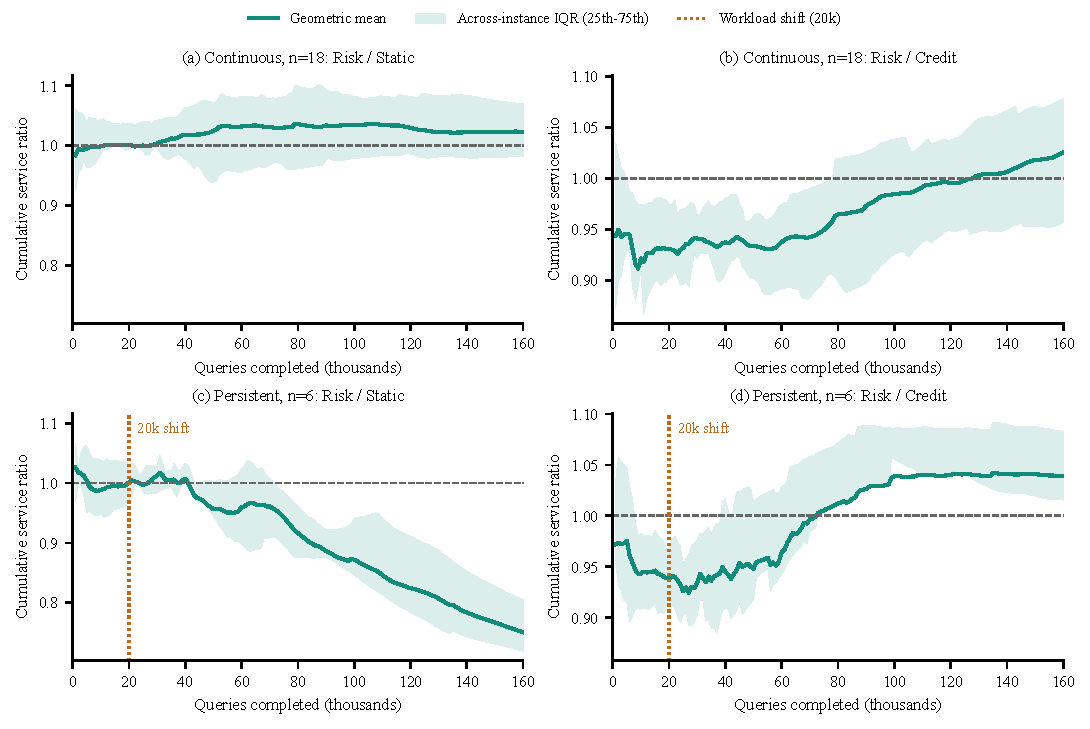
\includegraphics[width=.94\textwidth]{service_trajectories.pdf}
\caption{Cumulative service ratios.}
\label{fig:trajectories}
\end{figure*}

\subsection{Decision exposure and post-action opportunity}
\label{sec:mechanism}
Table~\ref{tab:decisions} partitions the 14,524 recorded decision boundaries; current-best and window-disagreement states share one logged category. At 13,473 boundaries the empirical tail test excludes at least one layout; in 7,620, the unconstrained mean-cost minimizer is excluded. These counts describe which choices the filter removes under the executed policy. At 364 of 1,205 confirmation- and cooldown-eligible price checks, the selected target's current evidence covers the forward-only threshold but remains below the installation-plus-return threshold. The controller produces 64 normal proposals and three repair proposals. One normal proposal is deferred by the byte budget; 63 normal replacements and three repairs execute. Credit-RePress and Horizon-RePress each record three budget deferrals, and every policy respects its payload cap. Joint policy comparisons quantify the resulting service and rewrite trade-offs.
\begin{table}[t]
\centering\small
\caption{Decision outcomes.}
\label{tab:decisions}
\begin{tabular}{@{}lr@{}}\toprule
Outcome & Boundaries \\
\midrule
Current best or window disagreement & 11,751 \\
Minimum gain test & 428 \\
Target confirmation & 1,137 \\
Evidence price & 1,141 \\
Proposed action & 67 \\
\midrule Total & 14,524 \\
\bottomrule\end{tabular}
\end{table}


For action $e$, let $I_e$ contain subsequent requests to its chunk through the query triggering the next replacement, or through the observed trace end. The triggering query of $e$ is served before that action. Post-action opportunity is
\begin{equation}
\widehat S_e=\sum_{t\in I_e}[\mu_{c_e}(r_e^-,x_t)-\mu_{c_e}(r_e^+,x_t)].
\label{eq:postaction}
\end{equation}
This is a counterfactual difference on the frozen calibration surface using the observed request sequence. We compare it with measured forward replacement time $M_e$ and unscaled calibrated price $P_e=m_{c_e}(r_e^-,r_e^+)+m_{c_e}(r_e^+,a_0)$. Admission applies the 1.25 margin to historical evidence in Eq.~\eqref{eq:admission}. Executed cost and calibrated price use distinct records: execution variability can place measured forward cost above the calibrated two-direction price. Episode coverage is evaluated at the last observed request; terminal episodes are right-censored at the trace end.
\begin{table*}[!t]
\centering\small
\caption{Post-action opportunity and cost.}
\label{tab:payback}
\begin{tabular}{@{}lrrrrr@{}}\toprule
Episode class & Episodes & $\widehat S_e\geq M_e$ & $\widehat S_e\geq P_e$ & Terminal & Median $\widehat S_e/M_e$ \\
\midrule
Continuous / normal & 20 & 14 & 12 & 17 & 1.56 \\
Continuous / repair & 3 & 0 & 0 & 3 & -16.53 \\
Persistent / normal & 43 & 40 & 41 & 43 & 6.30 \\
\bottomrule\end{tabular}
\end{table*}


In persistent shifts, 40 of 43 normal episodes have $\widehat S_e\geq M_e$, and 41 cover $P_e$; the median $\widehat S_e/M_e$ is 6.30. In continuous mixtures, 14 of 20 normal episodes cover $M_e$ and 12 cover $P_e$, with median ratio 1.56. Three normal episodes are closed by a return to the initial layout; one has modeled opportunity covering both executed replacements. The three repair episodes restore the empirically feasible reference and have negative mean-cost opportunity relative to the layouts they replace. Their measured costs remain in the service and rewrite totals. Model opportunity and realized service are complementary records: the latter also contains controller work and observed query-cost variation.

\subsection{Observed query tails and event tails}
Equation~\eqref{eq:feasible} concerns calibrated query-path distributions. The stable cohort contains 14,328 windows with 768 local requests under an unchanged layout and no migration at the decision boundary; 14,318 pass the model feasibility test. Table~\ref{tab:agreement} reports observed query and event p99 agreement within that model-feasible cohort; its last two columns count windows satisfying the 10\% paired tolerance. Agreement requires both the 256- and 768-query ratios to remain within 1.10. Paired ratios use identical requests from separately timed Static and Risk-RePress executions. The reference layout passes model feasibility by construction; separately timed queries still vary, and event timing also includes control work. Overlapping windows supply descriptive conditional counts; each workload instance remains the unit of the policy comparisons.
\begin{table}[t]
\centering\small
\caption{Tail agreement in stable windows.}
\label{tab:agreement}
\begin{tabular}{@{}lrrr@{}}\toprule
Layout & Model-feasible & Query p99 & Event p99 \\
\midrule
Reference & 11,851 & 6,084 & 3,967 \\
Adapted & 2,467 & 1,744 & 1,580 \\
\bottomrule\end{tabular}
\end{table}


The largest service ratio to Static occurs in the first group's 8K noisy-burst instance: 8.579 versus 7.410~s, with event p99 of 120.6 versus 99.2~$\mu$s. Its one migration costs 0.055~s, controller work costs 0.184~s, and query time differs by 0.931~s. These components preserve a concrete unfavorable instance alongside the aggregate comparisons.

\subsection{RQ3: Recovery across activation and retirement}
The new campaign contains 492 successful trials, summarized in Table~\ref{tab:recovery}. Controlled exceptions cover all 20 directed pairs over the original five layouts, both sizes, and ten software-visible stages. Additional checks exercise the 4,096-value layout in both directions against whole LZ4. Forty trials terminate the process directly. Twelve truncate the new payload after activation while the previous version remains retained. Reopening checks the active codec, exact values, query answers, catalog integrity, and repeated recovery.
\begin{table}[t]
\centering\small
\caption{Recovery test outcomes.}
\label{tab:recovery}
\begin{tabular}{@{}lrr@{}}\toprule
Trial class & Trials & Passed \\
\midrule
Controlled stage exceptions & 440 & 440 \\
Abrupt process exit & 40 & 40 \\
Post-activation payload truncation & 12 & 12 \\
\midrule Total & 492 & 492 \\
\bottomrule\end{tabular}
\end{table}

A separate abrupt-exit reproduction stops the original executor after old block metadata is deleted and before its cleanup transaction. Restart then raises a missing-metadata error while reconstructing the retained version. In the revised path, retirement has committed before this deletion stage; restart treats remaining old files as unreferenced garbage. The paired protocol trace and fault records bind this ordering to the executed implementation.

\section{Discussion}
\label{sec:discussion}
\subsection{What the coordinated mechanism controls}
The empirical tail filter defines candidate feasibility at decision boundaries. Feasible-epoch counters discard evidence when that condition fails, while installation-plus-return pricing accounts for the repair behavior induced by the criterion. The decision logs show both filtering exposure and price checks at which return cost changes eligibility. The policy comparison then measures the complete combination under a shared executor.

Risk-RePress's lower event p99 and rewriting relative to Credit-RePress accompany a service-time interval of 0.995--1.065. Against Static, persistent shifts and continuous mixtures occupy different operating regions. The post-action model analysis explains how much opportunity appears after accepted changes; measured service includes the actual query, controller, and maintenance components. The 10\% admission setting is interpreted on its calibrated query-path distribution, with query-window and event-window observations reported separately.

\subsection{Calibration reuse and lifecycle cost}
The storage component's commissioning process collects profiles before online adaptation. Credit-RePress and Risk-RePress use the same cost surface and directed replacement table, so that expenditure is common to their policy comparison. A fixed-layout deployment can use a smaller profiling procedure or a configured layout. Its incremental commissioning difference therefore depends on that deployment's selection process.

Let $\Delta T_{\mathrm{cal},b}$ and $\Delta T_{\mathrm{setup},b}$ denote additional commissioning and setup relative to baseline $b$. For $N$ queries over which the calibrated chunks remain reusable, a fixed-rate amortization condition is
\begin{equation}
N\overline{\Delta t}_b>
\Delta T_{\mathrm{cal},b}+\Delta T_{\mathrm{setup},b},
\label{eq:amortization}
\end{equation}
where $\overline{\Delta t}_b$ is average net service saving per request, including control and replacement. A positive saving and a sufficiently long reuse lifetime are both required. The reported 400.9~s covers all six eight-chunk calibration groups; each group's profile is reused across its workload instances.

As a conservative fixed-rate reuse scenario against Static, we assign the entire recorded group calibration to adaptation and zero commissioning to Static, then add the measured controller-setup difference. Holding each persistent-shift instance's measured net service saving fixed yields query-equivalent thresholds of 1.69--11.69 million requests per eight-chunk group, with median 5.45 million. This projection specifies its cost allocation and fixed saving rate; the source table also retains instances with non-positive measured savings. Calibration reuse is conditioned on the chunk bytes, candidate codecs, query kernels, and operating cache/hardware conditions. Cost changes call for refreshed profiles.

The commissioning view complements amortized analysis and profiling in runtime tuning and resource-sensitive scheduling \citep{alvarez2027online,wu2027sensascale}. Here the reuse unit is the calibrated physical chunk and layout configuration. Conditional-count tables add measured initialization and memory costs while reducing repeated online distribution work.

\subsection{Physical data and recovery scope}
The 48 distinct chunks contain 2.25~MiB of raw values and fit in memory. File-backed codecs, synchronized replacement, and catalog commits remain in execution. The measurements characterize this warm-file component on one Windows/NTFS host. Larger distinct corpora, other cache conditions, concurrent arrivals, and longer-term host variation provide additional deployment axes.

Recovery is organized around the active-pointer commit and retirement of the predecessor. The invariant table identifies the authoritative and retained versions at each boundary; 492 software-visible interruption and corruption trials check those cases. Hardware power interruption, device ordering, replica failover, and concurrent readers introduce additional scheduling and persistence conditions. Detailed development history, parameters, seeds, and hashes remain in the companion artifact, separate from the final scientific comparisons.

\FloatBarrier
\section{Related work}
\label{sec:related}
\subsection{Physical design and compression}
Automatic physical design selects database structures using workload information \citep{chaudhuri1997autoadmin,bruno2005physical}. Database cracking integrates reorganization with query execution \citep{idreos2007cracking}; self-driving systems extend automated decisions to broader configuration spaces \citep{vanaken2017ottertune,pavlo2017selfdriving}.

OReO studies online layout replacement through metrical task systems and dynamic layout generation \citep{rong2024oreo}. Its theoretical framework establishes the role of reorganization costs. RePressDB uses a finite codec/block space, directed measured transactions, and an empirical request-tail constraint. A common work-function-inspired baseline evaluates switching-cost logic in that measured action space.

AdaCom samples segment accesses and changes compression according to hot/cold behavior in DuckDB \citep{windheuser2024adacom}. Its memory/CPU trade-off complements the operation-dependent latency and durable replacement costs studied here. Compression-aware processing likewise links operators to encodings \citep{stonebraker2005cstore,abadi2006compression,damme2020morphstore}. Gorilla, BTrDB, and Sprintz demonstrate specialized time-series storage and compression designs \citep{pelkonen2015gorilla,andersen2016btrdb,blalock2018sprintz}. The present layout space exposes selective-decompression and summary-processing costs through general-purpose codecs.

Recent index-tuning work identifies structural query-plan changes associated with performance regressions \citep{wu2025qpr}. RePressDB's empirical latency filter addresses regression during physical adaptation at a different level: operation/length distributions over compressed chunks. It complements the average-cost criterion with a measured tail-risk reference.

\subsection{Runtime control and durable execution}
Self-adaptive architectures separate observation, analysis, planning, and actuation \citep{kephart2003vision,garlan2004rainbow,salehie2009landscape,delemos2013roadmap}. Stability and proactive adaptation studies emphasize decision cost, action frequency, and settling behavior \citep{salama2017stability,ayala2021prodspl,chen2024reliable}. Recent FGCS task tuning evaluates how analysis costs amortize over execution \citep{alvarez2027online}, while resource-sensitive scheduling connects constraints to system measurements \citep{wu2027sensascale}. These connections motivate including control and actuation inside service accounting.

Write-ahead logging, retained versions, and atomic visibility provide the recovery foundations \citep{mohan1992aries,gray1992transaction,sqlitewal}. RePressDB applies them to measured layout replacement, consolidating preparation updates and ordering retirement before deletion. The recovery case split identifies the software-visible stages used in fault injection, following the distinction between fault-tolerance mechanisms and their assessment \citep{avizienis2004dependability}.

\section{Conclusion}
RePressDB coordinates operation-dependent query distributions with empirical tail admission and recoverable physical replacement. Consecutive feasible decision epochs connect historical evidence to the current risk criterion, while directed installation-plus-return prices account for a later repair action. Exact conditional counts reduce online decision work, and three durable catalog transactions preserve activation and retirement ordering.

The common-executor evaluation exposes a specific trade-off: migrations fall from 155 to 66 and event p99 relative to cumulative-credit admission has ratio 0.872 (0.816--0.928), while the service-time ratio is 1.029 (0.995--1.065). Persistent shifts yield a 25.0\% service reduction against Static; continuous mixtures retain their observed event-tail cost. Decision records, post-action model opportunity, complete replacement measurements, and 492 successful software-fault tests connect these results to the executed mechanism. Calibration reuse and the measured data/cache conditions define the lifecycle in which these operating choices can be assessed.

\section*{CRediT authorship contribution statement}
\textbf{Zhichao Zhang}: Conceptualization; Methodology; Software; Formal analysis; Investigation; Validation; Data curation; Visualization; Project administration; Supervision; Writing -- original draft; Writing -- review and editing. \textbf{Daoqi Sun}: Formal analysis; Investigation; Validation; Visualization; Writing -- review and editing. \textbf{Xiaolu Peng}: Software; Investigation; Validation; Data curation; Resources; Writing -- review and editing.
\section*{Data and code availability}
The public datasets are available from the cited sources. The companion reproducibility archive contains the revised experiment driver, unchanged original measurement sources with SHA-256 provenance, protocol and environment records, calibration observations, per-instance summaries, migration records, event-latency arrays, and manuscript-generation code. The earlier artifact is available at \url{https://github.com/Jasper-Cheung/RePressDB-Artifact}. The revised archive identifies which results are newly measured and which are archival.
\section*{Declaration of competing interest}
The authors declare that they have no known competing financial interests or personal relationships that could have appeared to influence the work reported in this paper.
\section*{Funding}
This research received no specific grant from funding agencies in the public, commercial, or not-for-profit sectors.
\section*{Acknowledgements}
The authors acknowledge the maintainers of the public PEMS and Building Data Genome Project~2 datasets.
\bibliographystyle{elsarticle-num}
\bibliography{references}
\end{document}
